% !TeX spellcheck = da_DK
\subsection{Offsetjustering}
\subsubsection{Teori og design}
Det analoge signal, der kommer fra accelerometeret, har et indbygget offset på halvdelen af dens spændingsforsyning. For at kunne forstærke signalet der både skal indeholde positive og negative værdier, er det nødvendigt at ændre dette offset. På denne måde kan  accelerometeret i steady state have et outputsignal på $0$V. Måden dette nye offset indføres er ved anvendelse af et differensforstærker kredsløb. Dette kredsløb kan tage et af inputsignalerne og  fratrække det  andet inputsignal. Kredsløbet designes således:

\begin{figure}[H]
\centering
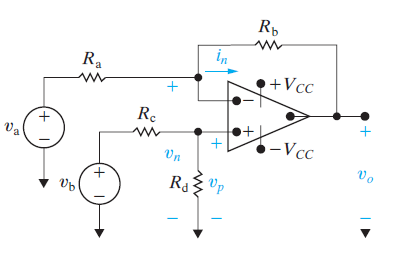
\includegraphics[scale=1]{figures/cProblemloesning/Differensforstaerker_generisk.png}
\caption{På figuren er et generisk differensforstærker kredsløb illustreret \ref{Nilsson2011}.}
\label{fig:Differensforstaerker_generisk}
\end{figure}

Ligning \ref{eq:Diff1} er den simplificeret ligning for differensforstærker kredsløbet, hvor $\frac{R_a}{R_b} = \frac{R_c}{R_d}$;

\begin{equation}\label{eq:Diff1}
V_o = \frac{R_b}{R_a} \cdot (v_b - v_a)
\end{equation}

Det kan heraf ses at forstærkningen på signalet kan bestemmes ved at vælge modstandene $R_a \text{og} R_b$ og at det er spændingsforsyningen $v_a$ der trækkes fra spændingsforsyningen $v_b$. 

I dette tilfælde kræves der ikke en forstærkning, derfor skal modstandene $R_{a}$ og $R_{b}$ være det samme. Da signalet ikke skal inverteres sættes accelerometerets output ind i den ikke-inverterende kanal og offsettet, som i dette tilfælde er på $1.5915$V jævnført  \ref{Mean_tid_0g} på side \pageref{Mean_tid_0g}, ind i den inverterende kanal. Dette illustreres på figur \ref{fig:Offset_generisk}:
\begin{figure}[H]
\centering
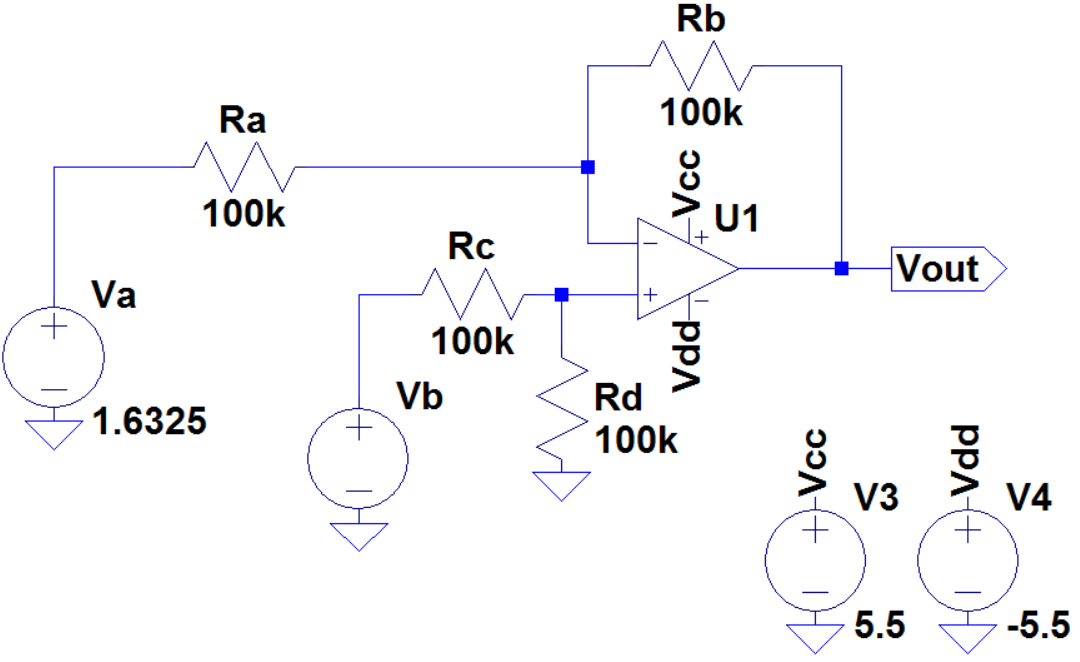
\includegraphics[scale=1]{figures/cProblemloesning/Offset_generisk.png}
\caption{På figuren ses offsetjusteringen, hvor V$1$ er det nuværende offset på accelerometeret og Va er outputtet fra accelerometeret. Modstandene i kredsløbet er alle ens, hvilket medføre at signalet ikke forstærkes. Grunden til at spændingsforsyningen er $\pm 6$V er at spændingsforsyningen til hele systemet, er designet til at give et output på $\pm 6$V.}
\label{fig:Offset_generisk}
\end{figure}

\subsubsection{Simulering}
Ved simulering i LTspice af kredsløbet som vist på \figref{fig:Offset_generisk} er outputtet fra accelerometeret (Va), sat til at være $1.60$V, og offsettet (V$1$) er på accelerometeret $1.5915$V. Derfor det forventet output af blokken være bestemt ved følgende udregning: 

\begin{equation}
\begin{aligned}
V_{out}={} & Va - V1 \\
           & 1.60V - 1.5915V \\
           &  0,0085V = 8.5mV
\end{aligned}
\end{equation}

Resultat er lig med værdien, der fremkommer ved simuleringen i LTspice som fremgår af \figref{fig:Offset_simulering}. Dette betyder at kredsløbet fungere rent teoretisk med ideelle komponenter, som bliver brugt i LTspice.  
\begin{figure}[H]
\centering
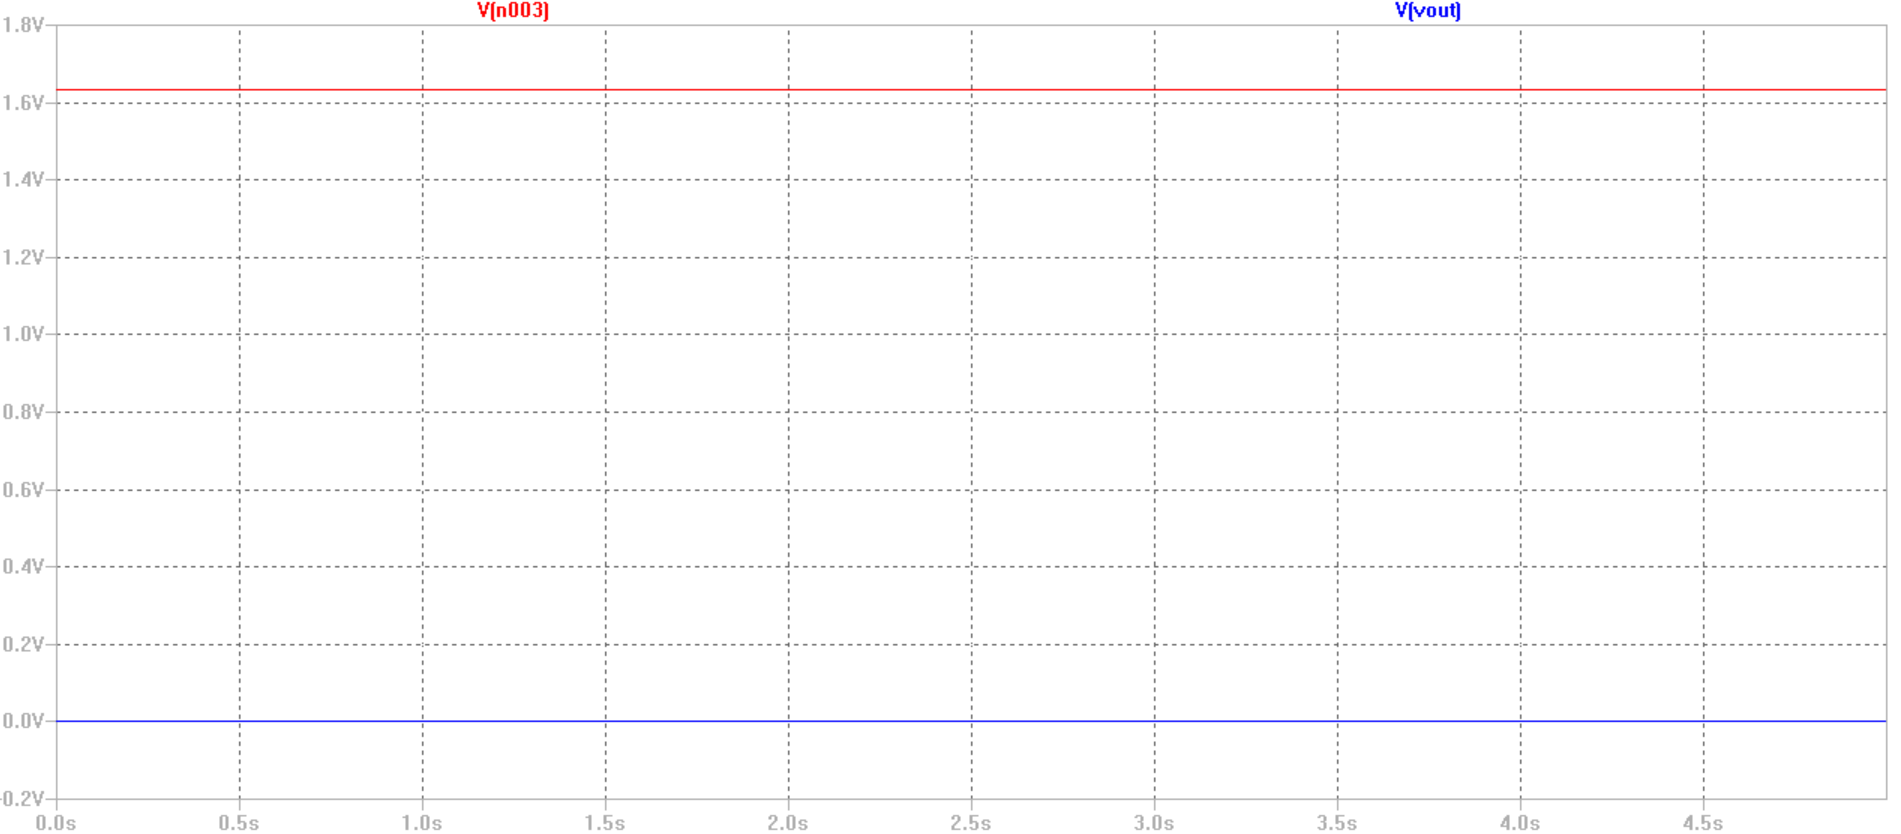
\includegraphics[scale=0.7]{figures/cProblemloesning/Offset_simulering.png}
\caption{På figuren ses en simulering af kredsløbet}. 
\label{fig:Offset_simulering}
\end{figure}

\subsubsection{Implementering og test}